%% This is file `dvipdfmx.def' for DVIPDFMx by J.-H. Cho and S. Hirata
%% which is written based on `dvipdf.def' in the LaTeX `Graphics Bundle'.
%%
%% This is file `dvipdf.def',
%% generated with the docstrip utility.
%%
%% The original source files were:
%%
%% drivers.dtx  (with options: `dvipdf,color1,psrulesZ')
%% 
%% drivers.dtx Copyright (C) 1994      David Carlisle Sebastian Rahtz
%%             Copyright (C) 1995 1996 1997 1998 1999 David Carlisle
%%
%% This file is part of the Standard LaTeX `Graphics Bundle'.
%% It may be distributed under the terms of the LaTeX Project Public
%% License, as described in lppl.txt in the base LaTeX distribution.
%% Either version 1.0 or, at your option, any later version.
%%
\ProvidesFile{dvipdfmx.def}
        [1999/02/16 v3.0i Driver-dependant file (DPC,SPQR)]
\def\c@lor@arg#1{%
  \dimen@#1\p@
  \ifdim\dimen@<\z@\dimen@\maxdimen\fi
  \ifdim\dimen@>\p@
    \PackageError{color}{Argument `#1' not in range [0,1]}\@ehd
  \fi}
\def\color@gray#1#2{%
  \c@lor@arg{#2}%
  \edef#1{[#2]}%
  }
\def\color@cmyk#1#2{\c@lor@@cmyk#2\@@#1}
\def\c@lor@@cmyk#1,#2,#3,#4\@@#5{%
  \c@lor@arg{#4}%
  \c@lor@arg{#1}%
  \c@lor@arg{#2}%
  \c@lor@arg{#3}%
  \edef#5{[#1 #2 #3 #4]}%
  }
\def\color@rgb#1#2{\c@lor@@rgb#2\@@#1}
\def\c@lor@@rgb#1,#2,#3\@@#4{%
  \c@lor@arg{#1}%
  \c@lor@arg{#2}%
  \c@lor@arg{#3}%
  \edef#4{[#1 #2 #3]}%
  }
\def\color@RGB#1#2{\c@lor@@RGB#2\@@#1}
\def\c@lor@@RGB#1,#2,#3\@@#4{%
 \c@lor@RGB@rgb{#1}\@tempa
 \c@lor@RGB@rgb{#2}\@tempb
 \c@lor@RGB@rgb{#3}\@tempc
 \c@lor@@rgb\@tempa,\@tempb,\@tempc\@@#4%
  }
\def\c@lor@RGB@rgb#1#2{%
  \dimen@#1\p@
  \divide\dimen@\@cclv
  \edef#2{\strip@pt\dimen@}}
\def\color@hsb#1#2{\c@lor@@hsb#2\@@#1}
\def\c@lor@@hsb#1,#2,#3\@@#4{%
  \c@lor@arg{#1}%
  \c@lor@arg{#2}%
  \c@lor@arg{#3}%
  \edef#4{[#1 #2 #3] hsb}%
  }
\def\color@named#1#2{\c@lor@@named#2,,\@@#1}
\def\c@lor@@named#1,#2,#3\@@#4{%
  \@ifundefined{col@#1}%
    {\PackageError{color}{Undefined color `#1'}\@ehd}%
  {\edef#4{ #1}}%
  }
\def\c@lor@to@ps#1 #2\@@{\csname c@lor@ps@#1\endcsname#2 \@@}
\def\c@lor@ps@#1 #2\@@{TeXDict begin #1 end}
\def\c@lor@ps@rgb#1\@@{#1 setrgbcolor}
\def\c@lor@ps@hsb#1\@@{#1 sethsbcolor}
\def\c@lor@ps@cmyk#1\@@{#1 setcmykcolor}
\def\c@lor@ps@gray#1\@@{#1 setgray}
\def\current@color{[0]}
\def\set@color{%
            \special{pdf:bcolor \current@color
                          }\aftergroup\reset@color}
\def\reset@color{\special{%
         pdf:ecolor}}
\def\set@page@color{\special{%
         pdf:bgcolor \current@color}}
\def\define@color@named#1#2{%
  \expandafter\let\csname col@#1\endcsname\@nnil}
\def\Ginclude@eps#1{%
 \message{<#1>}%
  \bgroup
  \def\@tempa{!}%
  \dimen@\Gin@req@width
  \dimen@ii.1bp%
  \divide\dimen@\dimen@ii
  \@tempdima\Gin@req@height
  \divide\@tempdima\dimen@ii
    \special{PSfile="#1"\space
      llx=\Gin@llx\space
      lly=\Gin@lly\space
      urx=\Gin@urx\space
      ury=\Gin@ury\space
      \ifx\Gin@scalex\@tempa\else rwi=\number\dimen@\space\fi
      \ifx\Gin@scaley\@tempa\else rhi=\number\@tempdima\space\fi
      \ifGin@clip clip\fi}%
  \egroup}
\def\Ginclude@bmp#1{%
 \message{<#1>}%
  \bgroup
  \def\@tempa{!}%
    \special{pdf:image\space
      width  \the\Gin@req@width\space
      height \the\Gin@req@height\space
      (#1)}%
  \egroup}
\def\Grot@start{%
\special{pdf:btrans rotate \Grot@angle}}
\def\Grot@end{\special{pdf:etrans}}
\def\Gscale@start{%
\special{pdf:btrans xscale \Gscale@x\space yscale \Gscale@y}}
\def\Gscale@end{\special{pdf:etrans}}
\def\Gin@PS@raw#1{\special{ps: #1}}
\def\Gin@PS@restored#1{\special{" #1}}%"
\def\Gin@PS@literal@header#1{\AtBeginDvi{\special{! #1}}}
\def\Gin@PS@file@header#1{\AtBeginDvi{\special{header=#1}}}
\@namedef{Gin@rule@.jpg}#1{{bmp}{.bb}{#1}}
\@namedef{Gin@rule@.jpeg}#1{{bmp}{.bb}{#1}}
\@namedef{Gin@rule@.png}#1{{bmp}{.bb}{#1}}
\@namedef{Gin@rule@.bmp}#1{{bmp}{.bb}{#1}}
%\def\Gin@extensions{.eps,.ps,.eps.gz,.ps.gz,.eps.Z}
\def\Gin@extensions{.jpg,.jpeg,.png,.bmp,.pdf,.eps,.ps,.eps.gz,.ps.gz,.eps.Z}
%\@namedef{Gin@rule@.pdf}#1{{bmp}{.bb}{#1}}
\@namedef{Gin@rule@.pdf}#1{{eps}{.bb}{#1}}
%
\@namedef{Gin@rule@.ps}#1{{eps}{.ps}{#1}}
\@namedef{Gin@rule@.eps}#1{{eps}{.eps}{#1}}
\@namedef{Gin@rule@.pz}#1{{eps}{.bb}{`gunzip -c #1}}
\@namedef{Gin@rule@.eps.Z}#1{{eps}{.eps.bb}{`gunzip -c #1}}
\@namedef{Gin@rule@.ps.Z}#1{{eps}{.ps.bb}{`gunzip -c #1}}
\@namedef{Gin@rule@.ps.gz}#1{{eps}{.ps.bb}{`gunzip -c #1}}
\@namedef{Gin@rule@.eps.gz}#1{{eps}{.eps.bb}{`gunzip -c #1}}
\@namedef{Gin@rule@*}#1{{eps}{\Gin@ext}{#1}}
\endinput
%%
%% End of file `dvipdfmx.def'.


\begin{filecontents*}{8.6.tex}
%#!F=hoge; platex $F.tex && dvipdfmx $F && open $F.pdf 
\documentclass[10pt,dvipdfmx,papersize]{jsarticle} 
\usepackage{type1cm,multicol} 
\usepackage{color} 
\pagestyle{empty} 
\begin{document} 
\renewcommand \DefineNamedColor[4]{% 
\textcolor[#3]{#4}{\rule{2em}{1em}}\space{#2}\\} 
\parindent=0pt 
\begin{multicols}{3} 
\input{dvipsnam.def} 
\end{multicols} 
\end{document} 
\end{filecontents*}

\begin{filecontents*}{jou-app.dic}
中括弧		ちゅうかっこ
丸括弧		まるかっこ
任意引数	にんいひきすう
例題		れいだい
処理速度	しょりそくど
前方参照	ぜんぽうさんしょう
原稿中		げんこうちゅう
参照		さんしょう
命令		めいれい
問題		もんだい
図表番号	ずひょうばんごう
変数		へんすう
天地		てんち
定数		ていすう
定義		ていぎ
宣言型		せんげんがた
小口		こぐち
引数		ひきすう
後方参照	こうほうさんしょう
必須引数	ひっすひきすう
書体		しょたい
机上組版	きじょうくみはん
波括弧		なみかっこ
版面		はんめん
環境		かんきょう
相互参照	そうごさんしょう
端末		たんまつ
節見出し	せつみだし
組版		くみはん
角括弧		かくかっこ
言語		げんご
関数		かんすう
大括弧		だいかっこ
書籍作成	しょせきさくせい
原稿執筆	げんこうしっぴつ
編集		へんしゅう
校正		こうせい
面付け		めんつけ
印刷		いんさつ
裁断		さいだん
製本		せいほん
型コマンド	かたこまんど
活版印刷	かっぱんいんさつ
字面		じづら
原稿		げんこう
抽象化		ちゅうしょうか
小括弧		しょうかっこ
警告		けいこく
執筆支援環境	しっぴつしえんかんきょう
禁則処理	きんそくしょり
選択		せんたく
入れ替え	いれかえ
集約		しゅうやく
終端記号	しゅうたんきごう
手続き		てつづき
展開		てんかい
下位		かい
小節		しょうせつ
文献		ぶんけん
今後の課題	こんごのかだい
付録 		ふろく
先行研究 	せんこうけんきゅう
全体の見通し 	ぜんたいのみとおし
分割する 	ぶんかつする
列の折り返し 	れつのおりかえし
列指定子 	れつしていし
前付け		まえつけ
参考文献 	さんこうぶんけん
大規模文書 	だいきぼぶんしょ
奥付 		おくづけ
妥当性の検証 	だとうせいのけんしょう
学位論文 	がくいろんぶん
実験と評価 	じっけんとひょうか
実験		じっけん
将来の展望 	しょうらいのてんぼう
序論 		じょろん
後付け 		あとづけ
意識 		いしき
折り返し 	おりかえし
拡張子 		かくちょうし
提案する理論 	ていあんするりろん
改ページ 	かいぺーじ
改丁 		かいちょう
数字 		すうじ
文脈 		ぶんみゃく
期待される効果 きたいされるこうか
本文 	       ほんもん
本論 	       ほんろん
概念的構造     がいねんてきこうぞう
概要 	       がいよう
用語集 	       ようごしゅう
番号 	       ばんごう
目次 	       もくじ
研究目標       けんきゅうもくひょう
研究補助者     けんきゅうほじょしゃ
研究費の提供者 けんきゅうひのていきょうしゃ
章毎にファイルを分ける	しょうごとにふぁいるをわける
章毎に分割 	しょうごとにぶんかつ
系		けい
索引 		さくいん
結言 		けつげん
結論 		けつろん
考察 		こうさつ
背景 		はいけい
表紙 		ひょうし
謝辞 		しゃじ
関連研究 	かんれんけんきゅう
題名 		だいめい
\end{filecontents*}

\begin{filecontents}{jou-app.ist}
lethead_flag            1
symhead_positive	"数字/記号"
letter_head		2
delim_0			" \\dotfill\\ "
delim_1			" \\dotfill\\ "
delim_2			" \\dotfill\\ "
lethead_prefix "\n\\underline{\\hbox to \\linewidth{\\large{\\sffamily\\bfseries "
lethead_suffix "\\hfill}}}\\nopagebreak\n"
\end{filecontents}

\begin{filecontents}{jou-app.map}
rml	H	HiraMinPro-W3
rmlv	V	HiraMinPro-W3
gbm	H	HiraKakuPro-W3
gbmv	V	HiraKakuPro-W3
\end{filecontents}

\documentclass[dvipdfmx,papersize]{jsarticle}
\usepackage{makeidx,type1cm,okumacro,url,graphicx,color,multicol,example}
\makeindex
% 解答
\newcounter{ksec}
\newcounter{kaito}[ksec]
\renewcommand\thekaito{\theksec.\arabic{kaito}}
\newcommand*\appkaito{\setcounter{ksec}{1}\def\theksec{\Alph{ksec}}}
% 章毎の解答の見出し
\newcommand*\kaitomidasi[1]{%
  \refstepcounter{ksec}\subsection{#1}}
% 解答
\newcommand\kaito[1]{%
\setcounter{kaito}{#1}\item[解答~\thekaito]}
% 索引にも追加する語句
\newcommand*\G[1]{\index{#1}#1}
% 語句
% \yougo{<語句>}{<英語表記>}{<関係する節>}
\newcommand*\yougo[3]{\index{#2}\index{#1@#1 (#2)}%
  \item[{\gtfamily #1}]#2\space(#3)\quad}
% 用語集の見出し
\newcommand*\yougohead[1]{\par
  \centerline{\gtfamily\large #1}\par\vskip\fboxsep
  \hrule\par\vskip.1\cvs}
% ファイル名
\newcommand*\fl[1]{\index{ファイル!#1@\texttt{#1}}\texttt{#1}}
% \LaTeX コマンド
\newcommand*\cmd[1]{\index{#1@\texttt{\protect\BS#1}}\texttt{\BS#1}}
% 環境型コマンド
\newcommand*\env[1]{\index{#1@\texttt{#1 環境}}\texttt{#1} 環境}
% 索引 3 段組用
\addtolength{\fullwidth}{1sp}
\addtolength{\textheight}{3\cvs}
\addtolength{\topmargin}{-3\cvs}
\addtolength{\footskip}{\cvs}
\begin{document}

\onecolumn

\title{『好き好き\LaTeXe 初級編』の補足・解答・用語集}
\author{渡辺徹\thanks{\texttt{http://mytexpert.sourceforge.jp/}}
  \thanks{thormac(at)gmail(dot)com}}
\date \today
\maketitle
\begin{abstract}
 「問題に解答がないと分かり辛い」というご意見がありましたので,解答を配
 布する事としました.略解は原稿中のコメントにその記述があります.
 本来であれば一つの書籍で完結させるべきだと思いますが,初学者が複数の選
 択肢を閲覧できるような冗長な記述は避けたいと感じていました.さらに,従
 来の \TeX の世界における用語の扱いについても疑問を抱いておりました.
 ``cross reference''はクロス参照と訳するのは適切ではないだろうし,かといっ
 て相互参照では直感的な理解に欠ける…という討論を頭の中で続けておりまし
 た.その結果,類書の用語とは異なる言い回しや表現が比較的多くなったと思
 いますので,対応表のようなものも作成する必要があると判断しました.
 日常的用語,慣習的用語ではうまく表現できないと判断したものには,新しく
 用語を作っている物もあります.
 以下,『本文書』という表現を『好き好き\LaTeXe 初級編』及び『学生・研究
 者・科学者のための\LaTeX を用いた論文作成術』として扱います.
\end{abstract}
%\maketitle
\tableofcontents
\clearpage
\twocolumn

\section{問題解答}

\kaitomidasi{執筆を始める前に}
問題はありません.

\kaitomidasi{\LaTeX の基本}
\begin{description}
\kaito {1}
 どのような文章例でも良いでしょう.憲法序文でも構いません.タイプセット
 した時にエラーや警告が出たならば,そのエラー・警告が表示されている行を
 よく観察して,何が原因かを考えてみてください.

\kaito{2}
 実際には Easy\TeX とか \TeX Shop のような\G{執筆支援環境}を使ってしまえ
 ば,このような冗長な操作は必要ないでしょう.「なぜ\LaTeX を使いたいだけ
 なのに,CUI環境のコマンドなんて覚えなければならないんだ」と思われる方も
 多いと思います.しかし,\TeX の根本的な部分はいまだに伝統的なインタフェー
 スしか提供していません.後付けでGUI環境で操作できる\G{フロントエンド}を
 他の作者が開発しているに過ぎません.このような操作が出来ると後々便利な
 こともありますので,試しに実際に打ち込んでみてください.

\kaito{4}
非常に簡単なファイル,
\begin{verbatim}
\documentclass{jbook}
\listfiles
\begin{document}
 test
\end{document}
\end{verbatim}
をタイプセットしただけでも,
\begin{description}
\item[\fl{pldefs.ltx}] もっとも基本となる定義がなされたファイル
\item[\fl{jy1mc.fd}] 横組用明朝ファミリーに関する書体定義
\item[\fl{jy1gt.fd}] 横組用ゴシックファミリーに関する書体定義
\item[\fl{jt1mc.fd}] 縦組用明朝ファミリーに関する書体定義
\item[\fl{jt1gt.fd}] 縦組用ゴシックファミリーに関する書体定義
\item[\fl{kinsoku.tex}] \G{禁則処理}に関する設定ファイル
\item[\fl{plpatch.ltx}] \pLaTeX のパッチファイル
\item[\fl{jbook.cls}] \G{書籍作成}用文書クラスファイル
\item[\fl{jbk10.clo}] 基本となるフォントサイズを10\,ptで版面を設定するた
	     めのファイル
\end{description}
というファイルが読み込まれています.つまり,自分が意図したことよりも多く
の処理が裏でなされているという事になります.

\kaito{5} 最近はあまり \G{psutils} も使われなくなって来たのではないでしょう
 か.私もほとんど使っておりません.正式名称は \G{PostScript Utilities}だ
 と思います.以下のプログラムが含まれていますが,これら以外にもスクリプ
 ト類が付属する場合もあります.
\begin{description}
  \item[psbook] 面付けがしやすいようにページを入れ替えます.
  \item[psselect] 選択したページだけ抽出します.
  \item[pstops]  詳細な設定により入力PostScriptファイルから\G{面付け},
	     \G{ページ選択},\G{ページ入れ替え}を行ないます.
  \item[psnup] 複数のページを一枚に\G{集約}します.
  \item[psresize] \G{ページサイズ}を変更します.
  \item[psmerge] 複数のPostScriptファイルを結合します.
  \item[epsffit] \G{EPSFファイル}の\G{bounding box}を指定された物に変更
	     します.
\end{description}
\end{description}

\kaitomidasi{文章の書き方}
\begin{description}
\kaito {3}
一人の場合,簡単には次のようになるでしょう.
\begin{verbatim}
 \maketitle{一人目}
\end{verbatim}
実は,\LaTeX の内部において \cmd{maketitle} は次のような
仕組みで出力されています.
\begin{verbatim}
 \begin{tabular}[t]{c}
一人目
\end{tabular}
\end{verbatim}
このため,複数行にしたい時には単純に \verb|\\| を入力すれば
良い事になります.では,三人の場合はどうなるでしょうか.
\begin{verbatim}
\maketitle{一人目 \and 二人目 \and 三人目}
\end{verbatim}
これは \cmd{and} が\env{tabular}の終わりと始めを宣言すれば良いという事にな
ります.
\begin{verbatim}
\begin{tabular}[t]{c}
一人目\end{tabular}\begin{tabular}[t] 
一人目\end{tabular}\begin{tabular}[t] 
一人目
\end{tabular}
\end{verbatim}
このようにして著者名の上部を整列の基準として横に並べるのを実現しています.

\kaito{5}
\cmd{parindent} と \cmd{parskip} を調整する事で,段落始めの字下げなし・
段落間の空きによる段落分けという設定が可能ですが,通常は使わない方が良い
と思います.紙面ではなく,電子形式のみによる文書配布ではあり得るかもしれ
ません.このような設定にすると余計に紙面を食うので,資源に限りがある場
合は,\LaTeX における通常の設定のままで体裁を整えてください.

\kaito{6}
実際に入力例をタイプセットするだけで結果が分かります.
\end{description}



\kaitomidasi{コマンドとマークアップ}
\begin{description}
\kaito {1}
\cmd{newcommand} や \cmd{newenvironment} のように,新規に環境・宣言・
命令型のコマンドを定義すると,自動的に複数行の段落を引数として受けとる
ようになります.諸刃の剣だと私は思いますが,明らかに単一の段落しか受けと
らないようなコマンドであれば,アスタリスクを付与して定義しても良いと思い
ます.
複数の段落を受けとるという事は,\G{終端記号} (\G{terminator}) である閉じ
の波括弧を入れ忘れた場合,最悪原稿の末尾まで
そのコマンドに入力文字列が連れ去られる事になります.

\kaito{3}
\kenten{もろい} (\G{fragile}) コマンドと壊れにくい (\G{robust}) コマンドの例を示
しています.ほとんどのコンパイル型言語で言える事ですが,コンパイラはテキスト置換
しか内部で行なっていません.人間がどのような\G{オブジェクト}(\G{手続きやデータ})
をマクロや関数として\G{抽象化} (\G{abstraction}) したとしても,計算機内
 部では,ただの文字列に過ぎません.\TeX コンパイラは文字を紙面に組版する
 ために,文字列を\G{展開} (\G{expanding}) します.与えられた引数を逐次的
 に展開するか,どの引数を展開するか,という内部処理の問題をかいま見るた
 めの例題として結果も本書に載せています.ここでは\kenten{もろい}コマンド
 の中に\G{アットマーク} `@' が含まれているために,エラーが生じています.

\kaito{5} 
問題文では \cmd{thesection} だけを再定義しています.
\begin{verbatim}
\documentclass{jsarticle} 
\renewcommand\thesection{\Alph{section}} 
\begin{document} 
\tableofcontents 
\section{序論} 
\subsection{構成} 
\end{document} 
\end{verbatim}
しかし,これだけでは\G{下位のカウンタ}に対して再定義内容が波及していませんの
で,これとは別に対処が必要になります.\G{小節}にも節の体裁変更を適用する
には次のようにします.
\begin{verbatim}
 \renewcommand\thesubsection
    {\thesection.\arabic{subsection}}
\end{verbatim}

\end{description}

\kaitomidasi{数式の書き方}
\begin{description}
\kaito{1}
実際に入力し,その結果を吟味して頂ければご理解頂けると思われます.

\kaito{2} 
\env{eqnarray*}の中で次のようなエラーが生じします.
\begin{verbatim}
! LaTeX Error: Too many columns in 
               eqnarray environment.
\end{verbatim}
 \env{eqnarray}に許容できる以上の列が追加されている事を示します.これによ
 り3列まで整列させられる事が分かります.

\kaito{14}
解答略.

\kaito{15}
視覚的に違いはないと言って良いでしょう.内部では \env{array}の
中央揃えを用いている事と等価だと考えられます.

\kaito{16}
\cmd{multlinegap} は先頭行の空きを調整するためのコマンドである事が分かり
 ます.

\kaito{18}
解答略.

\kaito{19}
原稿中で頻出する数学関数は全て \cmd{DeclareMathOperator} で定義して
おくと便利だと思います.局所的にしか使用しない場合でも \cmd{operatorname}
を補うようにすると,適切な空白が補われます.

\kaito{20}
 要するに \env{array}を使っていると考えて良い訳ですから,垂直方向の
 揃えが変更されます.といっても,それほど使用頻度が高い訳ではないと思い
 ますが.
\end{description}

\kaitomidasi{図表の構成}
\begin{description}
\kaito{2} 
\cmd{maketitle} と \cmd{and} がどのように定義されているかを解説する物で
す.このようなテクニックは他に適用できるパターンがありそうです.

\kaito{5} 文章幅に応じて,張り込む画像の大きさを変更したい時に,
\cmd{linewidth} を使うと大変便利です.特に 2 段組の場合の文章では,
段の幅一杯に画像を拡大したい時があります.\cmd{includegraphics}
の width オプションに \cmd{linewidth} を入れてあげれば,それだけ
で微調整などが不要になります.
\begin{verbatim}
\includegraphics[width=\linewidth]
   {images/filename.pdf}
\end{verbatim}

\kaito{10}
`pa'というのがパスを追加するコマンドです.このパスに対して実線を描くのが
 `fp',塗りつぶしのための`ip',破線を描く`da',点線を描く`dt',スプライ
 ン曲線を描画する`sp'などがあります.`sh'というのが塗りつぶしを指定する
 ためのコマンドになります.

\kaito{11}
何十年も前に開発された描画用プログラム \textsc{PIC} です.いまは
\textsc{PIC}よりも便利な描画プログラムが沢山あると思います.
\end{description}

\kaitomidasi{文献一覧の作成}
\begin{description}
\kaito{1}
なぜかCコンパイラの話が出てきますが,とにかく,相互参照がうまく行くまで
\TeX ではタイプセットを複数回行なわなければなりません.

\kaito{2}
 アスタリスクを指定すると『\G{文献データベース}中にある全てのエントリ』
 を \cmd{nocite} した事となります(\G{ワイルドカード}として働きます).
詳しくは用語集『相互参照』を参照してください.
\end{description}


\kaitomidasi{\LaTeX の応用}
\begin{description}
\kaito{1}
解答略.

\kaito{2}
単に margin オプションに 2\,cm を指定するだけです.
\begin{verbatim}
 \geometry{margin=2cm}
\end{verbatim}

\kaito{3}
解答略.

\kaito{4}
解答略.

\kaito{6}
もしかしたら type1ec パッケージがないために,エラーになるかも知れません.
この場合は type1cm を使ってください.結果は次のようになります.
\begin{center}
 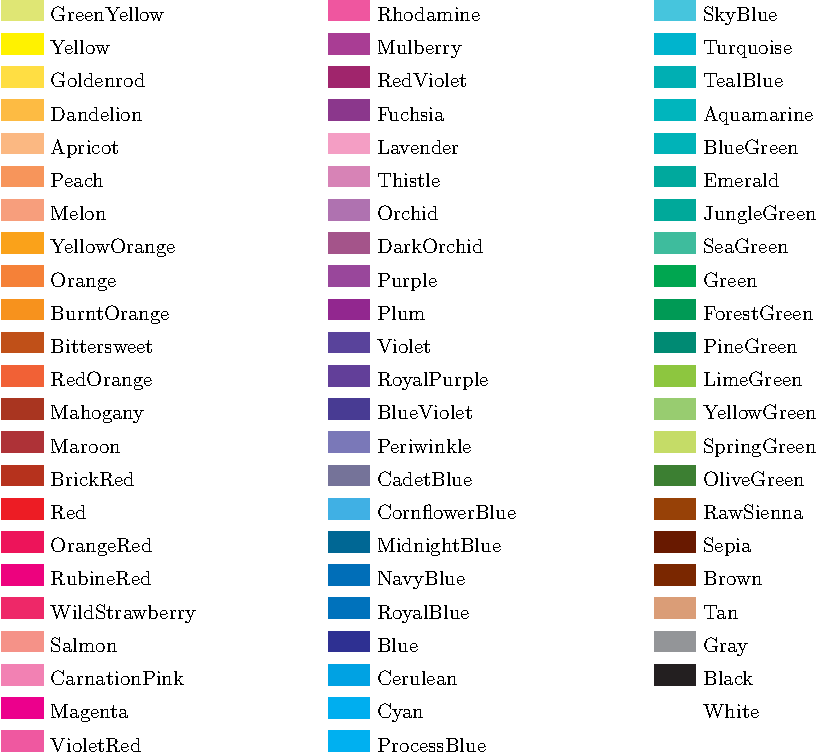
\includegraphics[bb=0 0 392 362,width=\linewidth]{8.6.pdf}
\end{center}

\kaito{9}
好みの問題もあると思いますので,適宜ご自分が良いと判断された設定を用いて
ください.

\kaito{10}
 どうやら例題と問題を書き間違えたようです.普通に入出力例を吟味してくださ
 い.

\kaito{11}
サンプルファイルはウェブ上からダウンロードできます.
\begin{verbatim}
tar zxvf mainsrc.tgz
cd mainsrc
make	
\end{verbatim}
まずは,上記のように実行してみてください.うまく行かなければ環境依存な記
述がある可能性もあります.\fl{main.tex}の文字コードが \G{EUC-JP} なので,
\G{UTF-8} 対応の \G{ptetex3} では platex-euc を実行する必要性があるかも
しれません.

\kaito{13}
入力例を実際にタイプセットすると結果が分かります.実数に対応させるために
は本書の解説だけでは実現するのが難しいと思います.こういう計算を得意とし
ているのはExcelのような表計算ソフトです.あまり \TeX でなんでも実現しよ
うと無理をしない方が歳を取らずに済みます.

\kaito{14}
結果は次のようになります.
\begin{quote}
\newcommand*\Qa[1]{\sqrt{a_{#1}} + }
\newcommand*\Qb[1]{\sqrt{b_{#1}} + }
$f = \Qa{1}\Qa{2}\Qa{3}\Qa{4}\Qa{5}\Qa{6}\Qa{7}\Qa{8}
\Qa{9}\Qa{10}\Qb{1}\Qb{2}\Qb{3}\Qb{4}\Qb{5}\Qb{6}\Qb{7}\Qb{8}\Qb{9}
\sqrt{b_{10}}$	
\end{quote}

\kaito{19}
解答略.

\end{description}

\kaitomidasi{文章のサンプル}
\begin{description}
\kaito{2}
節見出しの番号の後にピリオドが付与されます.場合によってはピリオドを付け
るような体裁にする事も良くあります.

\kaito{3}
`\cmd{par}\cmd{nobreak}' を削除すると章番号と見出しの間の改行が無くなり
 ます.\cmd{vskip}\cmd{Cvs} は垂直方向の空きが少なくなります.
`\cmd{raggedright}'は左揃えのコマンドですから`\cmd{centering}'にすると
中央揃えになります.

\kaito{4}
右余白が左余白と同様になります.左余白だけで引用を示す体裁もあれば,右余
白も追加する引用の体裁もあります.どちらが良いかは,慣習(と好み)に応じてください.

\kaito{5}
\cmd{leftskip} や \cmd{rightskip} は左右の空きを調整するためのコマンドで
 す.これらの記述を削除すると左右の余白があります.1\,cmでは余白が広い,
または狭いと感じた場合は \cmd{linewidth} を参照して次のように対処する事
 も出来ます.
\begin{verbatim}
\advance\leftskip  .05\linewidth
\advance\rightskip .05\linewidth
\end{verbatim}
 上記のように設定するとその段落における幅の5\%の余白を左右に追加する
 体裁となります.これにより1段組と2段組が混在するような場合でも多少なりと
 も見映えが良くなります.
 2006年9月以降のjsclassesではその段落における幅の6.28\%の余白を左右にそれ
 ぞれ挿入するように変更されました.

\kaito{6}
目次における章見出しの大きさに \cmd{large} が適用されて,一段階大きくな
ります.
\end{description}

\section*{付録Aの解答}
\appkaito
\begin{description}
 \kaito{3}
 \cmd{usepackage}コマンドに種々のパッケージを指定するだけで,基本書体の
 変更が簡単にできる事が実感できると思います.さらに,部分的にも全体的に
 も版面の印象が変わったり,文字の組まれ方が異なっている事と思います.

 \kaito{4}
解答略.
\end{description}

\section{用語集}

括弧内は関連する節番号を示す.

\yougohead{あ行}
\begin{description}
\yougo{イニシャルコマンド}{initial command}{2.1.7}
原稿の先頭部分,\cmd{documentclass} 命令が始まる前にしか記述できないコ
マンドの事です.

\end{description}
\yougohead{か行}
\begin{description}
\yougo{角括弧}{bracket}{2.1.8}
『\G{ブラケット}』または『\G{大括弧}』と呼ばれる事があります.
小括弧,中括弧,大括弧というのは分かり辛い,非直感的であるという指摘によ
り,本文書では一貫して角括弧としています.そもそも数式中では括弧の大きさ
を段階的に調整する事が可能で,ブレースを指し示す『大括弧』は大きくもな
り,小さくもなります.これにより,『角括弧』と書いた方が直感的であり一
貫性があると判断して`bracket'を訳しました.

\yougo{組版}{typesetting}{1.1}
「ある媒体,特に書籍などの紙のうえに読者が読みやすいように必要な情報を適
切な位置に配置する事」と本文中にありますが,伝統的には種々の\G{書体} (\G{types})
を適切な処理をして書籍の体裁及び書式を決定・調整 (setting) し,文字が並
んだ版を作成する事にあります.本来は活版印刷における活字を物理的に並べて
一枚の版を作成する行為を指します.
\G{書籍作成}には,\G{原稿執筆},\G{編集},\G{校正},\G{組版},
\G{面付け},\G{印刷},\G{裁断},\G{製本}という一連のプロセスがあります.
現代的広義の組版という用語は原稿執筆から校正(場合により面付け)までのプ
ロセスを含むと考えても良いと思います.

\yougo{コマンド}{command}{2.1.1}
類書においてもコマンドという用語で統一していると思います.
定義によっては「\G{宣言型コマンド}」「\G{命令型コマンド}」「\G{環境型コ
マンド}」というように,三つに分けている場合もあります.

\end{description}
\yougohead{さ行}
\begin{description}
\yougo{相互参照}{cross reference}{4.5}
『相互参照』とか,そのまま『\G{クロス・リファレンス}』と表記する事が
多いです.多少ではありますが『\G{クロス参照}』とする書籍もある.\TeX に限らず一般的
な\G{コンパイラ}は,ある要素に\G{ラベル}を付与し,そのラベルを参照する時に
後方か前方かによって(\G{プリプロセッサ}が判断して)コンパイル回数を調整
します.伝統的\G{C言語}のコンパイラであれば,後方参照 (backword
 reference) は許容されておらず,
 \G{マクロ}・\G{定数}・\G{変数}・\G{関数}の\G{定義}はラベルを使用する地
 点よりも前方に位置しなければなりませn.\G{前方参照} (\G{forward reference})
 のみという事は\G{処理速度}がそれだけ早い事になります.
\TeX もマクロや変数に関しては\G{後方参照}が認められていませんが,
『\G{カウンタ変数}』だけは(複数回のタイプセットを行なう事で)後方参照で
 きるような仕組みになっています.そのた
 め,\G{節見出し}や\G{図表番号}におけるカウンタ変数のラベルは前後のいず
 れでも参照できるという点から,相互参照 (\G{cross reference}) という名称になっ
 ているものと思います.

\yougo{書体}{typeface}{1.1}
書体とは文字 (\G{type}) の系統・様式の事です.\G{活版印刷}における
活字の\G{字面} (\G{face}) の種類を示すと考えて良いと思います.

\yougo{ソースファイル}{source file}{2.1.1}
文書の本文と\LaTeX のコマンドを記述した原稿の事です.\LaTeX はコンパイル
型の言語であり,もとのファイルに直接修正を施す訳ではありませんので,
\G{原稿} (\G{source}) が必要になります.

\end{description}
\yougohead{た行}
\begin{description}
\yougo{タイプセット}{typeset}{2.1.1}
本書では \LaTeX の原稿から \TeX プログラムを介して成形された DVI ファイ
ルを生成する事です.本来は活版印刷における用語です.用語『組版』も参照し
てください.「タイプセットしてください」とあった場合は,platex コマンド
等を実行する事を示します.

\yougo{端末}{terminal}{2.1.2}
\G{ターミナル},\G{コンソール},\G{コマンドプロンプト}の総称です.
いかなる環境においても,文字のみによって\G{オペレーティングシステム}の
\G{カーネル}に対して処理を要求する\G{CUI}環境の事を示します.本書の大部
分では「コンソール」として表現されている場合が多いです.

\end{description}
\yougohead{な行}
\begin{description}
\yougo{波括弧}{brace}{2.1.8}
『\G{ブレース}』『\G{中括弧}』と呼ばれる事があります.
同様に,用語『角括弧』も参照してください.

\end{description}
\yougohead{は行}
\begin{description}
\yougo{プリアンブル}{preamble}{2.1.6}
\verb|\begin{document}| よりも前の部分の事を示します.この部分でしか使用
する事を許されていないコマンドを\G{プリアンブルコマンド}
 (\G{preamble command}) と呼びます.

\end{description}
\yougohead{ま行}
\begin{description}
\yougo{マークアップ}{mark-up}{1.6}
ある具体的なオブジェクトに対して,その上位の概念及び\G{概念的構造}を付与する
事を意味します.1.6節の例では『人類普遍の原理である』という文字列を
中央揃えにするために center タグ,\env{center}で括っています.これは
その文字列に対して視覚的な構造を表現している事になります.4章のコマンド
とマークアップ(手続きとデータの\G{抽象化})に関係する重要な概念です.

\yougo{丸括弧}{parentheses}{2.1.8}
『\G{パーレン}』または『\G{小括弧}』と呼ばれる事があります.
同様に,用語『角括弧』も参照してください.

\end{description}
%\yougohead{や行}
%\begin{description}
%
%\end{description}
\yougohead{ら行}
\begin{description}
\yougo{ログファイル}{log file}{2.1.2}
何か作業をした時に,部下は上司に対して簡単には「任務完了しました」の一言
だけで報告を終わらせます.「詳細は報告書にまとめておくように」と上司に言
われた時だけそのような文書をまとめると思います.\LaTeX において,その
報告書に該当するのがログファイル (\G{拡張子}が .log) です.ログファイルを読
むためには,ある程度の経験と知識が必要になります.実際には処理を実行してい
る時に出力される\G{警告}と\G{エラー}だけを注意するようにすると効
率的だと思われます.\LaTeX ではエラーになると(\G{interaction mode}であ
る限り)指揮官(タイプセットを命令した人間)に指示を求めてきます.
\end{description}
%\yougohead{わ行}
%\begin{description}
%
%\end{description}
% \yougo{<語句>}{<英語表記>}{<関係する節>}

\onecolumn

\section{補足}

\subsection{表紙の怪しい英文}

『好き好き\LaTeXe 初級編』の表紙には次の一文が大体的に表示されています.
\begin{quote}
\begin{center}
\begin{em}
 Love Love \LaTeX\\
 ---for all beginners at the entry level---\\
 by Thor Watanabe\\
 ``The \TeX book has good examples, problems, and jokes.''
\end{em}
\end{center}
\end{quote}
要するに優れた教科書には良い\G{例題}・\G{問題}・\G{ジョーク}がちりばめられている,
という事です.本書は例題と問題をある程度含めました.依然として満足できる量
ではないので,今後『問題』の数は増えるものと思います.ジョークに関しては,
多少ではありますが,\G{原稿中のコメント}に含めるようにしました.

\subsection{6.3節に追加する例題・問題}
表6.3には八つの\G{列指定子}が列挙されていますが,その内の `@', `p', `*' の使
い方についての解説・例題・問題がありませんので補足します.

`@'は縦一列に指定した要素を追加するものですから,例えば次のようになりま
す.

\begin{example}
 \begin{tabular}{lll@{\,個}}
  \hline
  名称   & 型番 & \multicolumn{1}{l}{個数}\\
  \hline
  たわし & TWS01 & 1000\\
  石けん & SP01  & 5000\\
  \hline
 \end{tabular}
\end{example}

\index{折り返し}
\index{列の折り返し}
次に `@' を使う例を示します.`@'を使うと,該当する列を指定した幅で折り返
すようになりますので,非常に長い説明をつける時に使用します.

\begin{example}
 \begin{tabular}{lp{10zw}}
  \hline
  項目 & 説明\\
  \hline
  ICBM   & 大陸間弾道ミサイル\\
  START2 & 第二次戦略兵器削減条約\\
  MIRV   & 複数個別誘導再突入体又は多弾頭独立目標再突入ミサイル\\
  SLBM   & 潜水艦発射弾道ミサイル\\
  \hline
 \end{tabular}
\end{example}

最後に `*' を使う例を示します.これを用いる必要性というのはないと思いま
すが,何度も同じ表現しかない列指定子を記述する場合には,意味が明瞭になる
と思います.

\begin{example}
 \begin{tabular}{|*{3}{lr|}}
  \hline
  名称 & 金額 & 名称 & 金額 & 名称 & 金額 \\
  \hline
  たわし & 300 & 長靴 & 5,000 & はさみ & 1,000\\
  洗濯板 & 3,000 & 靴べら & 500 & のり & 100\\
  洗濯機 & 100,000 & 靴下 & 100 & 包丁 & 5,000\\
  \hline
 \end{tabular}
\end{example}

即ちこれは,rl を3回繰り返して,rlrlrlとして列指定子を記述した事と同じに
なります.

\subsection{8.13節の補足}

\index{原稿を分割する}
\index{ファイルを分割する}
\index{章毎にファイルを分ける}
『原稿を複数のファイルに分ける』とありますが,これには問題を付けるべきで
あったと思います.9.2.1節も同様に,\G{大規模文書}の執筆方法に直接的に触れて
いる箇所がありません.

書籍や論文は大きく分けて四つに分ける事が出来ます.
\begin{description}
 \item[表 紙]   読者が一目で何についての文書かが明確に分かる1ページで構成
	    された\G{題名}情報.
 \item[前付け] \G{目次},\G{まえがき},\G{謝辞}を含む,本文とは直接的に関係のない要素.
 \item[本 文]   \G{序論},\G{本論},\G{結論}等の本文を構成し,その論理性・妥当性を立
	    証するために必ず必要となる要素.付録もここに属するが,付録で
	    ある事が明確になるように区別する.
 \item[後付け] \G{参考文献},\G{用語集},\G{索引},\G{奥付}などを含み,文書の付加
	    的情報.
\end{description}

上記の四つの部分は,それぞれ次の命令で出力又は範囲の宣言をする事が出来ま
す.ただし,\G{book系のクラスファイル}だけで,\G{report系のクラスファイル}には用
意されていません.
\begin{description}
 \item[\G{表紙}] \cmd{maketitle}.
 \item[\G{前付け}] \cmd{frontmatter} により,それ以降が前付け部分である事を
	    宣言する.\LaTeX では\G{ページ番号}が\G{ローマ数字}で表記される事に
	    なる場合が多い.
 \item[\G{本文}] \cmd{mainmatter} により,それ以降が本文である事を宣言する.
	    \LaTeX ではページン番号が\G{アラビア数字}で表記される事になる場
	    合が多い.
 \item[\G{後付け}] \cmd{backmatter} により,それ以降が本文である事を宣言する.
\end{description}
いずれの場合でも \cmd{cleardoublepae} 命令等で,\G{改丁}(奇数ページから次
のページを始めるように\G{改ページ})されます.

まず,(大規模な書籍や)\G{学位論文}の構成は次のようになります.

\begin{description}
 \item[\G{表紙} (\G{Cover page})] 題名,著者名,日付などを明瞭に伝えるための顔.
 \item[\G{概要} (\G{Abstract})] 本文全てを要約したもの.
 \item[\G{目次} (\G{Contents})] 見出しを列挙したもの.
 \item[\G{まえがき} (\G{Preface})] 本文とは直接的に関係のない予備知識を補足するための文章.
 \item[\G{序論} (\G{Introduction})] \G{背景},\G{文脈},\G{問題意識},\G{研究目標}を含んだ冒頭部分.
 \item[\G{関連研究} (\G{Related Work})] 調査した研究と自分の研究との差異.
 \item[\G{提案する理論} (\G{The body of Proposal})] 提案する理論等.
 \item[\G{実験と評価} (\G{Experiments and Evaluation})] 提案する理論の\G{妥当性の検証}.
 \item[\G{考察} (\G{Discussion})] 提案する理論が妥当かどうかを議論
	    し,\G{将来の展望}や\G{期待される効果}についての言及.
 \item[\G{結言} (\G{Conclusion})] \G{結論}と\G{今後の課題}.
 \item[\G{謝辞} (\G{Acknowledgement})] \G{研究費の提供者},\G{研究補助者}に対する敬意.
 \item[\G{付録} (\G{Apendix})] \G{実験データ}や\G{ソースコード}等,実験
	    の信頼性を保障するための補足資料.
 \item[\G{参考文献} (\G{References})] \G{先行研究}や関連する研究の裏付けと道しるべ.
\end{description}

順番は若干異なる場合があります.

\paragraph{例題}
上記の構成をそのまま一つのファイルで記述しようと思えば,次のようになりま
す.以下のファイルをコピー\&ペーストでも構いませんので,実際に
\fl{ronbun.tex}などのファイル名で保存し,タイプセットした結果を吟味してくださ
い.

\narrowbaselines
\begin{verbatim}
\documentclass[11pt,dvipdfmx,papersize]{jsbook}%
\usepackage{amsmath,amssymb,bm,verbatim,listings}%
\begin{document} 
\title{卒業論文\\
	コンクリートの流動性と硬化速度に関する研究}
\author{所属:工学部建築学科\\
	学生番号:120-333001\\
	氏名:佐藤 高橋\\
	指導教官:近藤 江崎}
\date{提出日:平成18年1月31日}
\maketitle 
\frontmatter% 前付 
\chapter{概要}
本研究はコンクリートの流動性と硬化速度の関係について考察するものである.
\chapter{はじめに}
挨拶のようなものをここに記述します.
\tableofcontents 
\listoffigures 
\listoftables 
\mainmatter% 本文 
%\doublespacing % 
\chapter{序言}
背景,文脈,問題意識,研究目標について言及する.
\chapter{関連研究}
研究領域の詳細説明と関連研究の紹介をする.
\chapter{提案する理論}
提案する理論について言及する.
\chapter{実験と評価}
理論の妥当性を検証するための手法と評価方法.
\chapter{考察}
なぜ,それが妥当だと判断されるのかの根拠と,将来の展望など.
\chapter{結言}
結論と,今後の展開.
%\singlespacing % 
\begin{appendix}% 付録	
\chapter{ソースコード}
\end{appendix}% 
\backmatter% 後付 
\chapter{謝辞}
実験補助者,指導教官,研究費補助者に対する敬意.
\bibliographystyle{jplain}% 文献形式 
\bibliography{ron}% 参考文献 
\end{document} 
\end{verbatim}

\paragraph{問題}

\widebaselines
しかし,単一のファイルに全ての内容を記述すると,膨大な量になり,語句の検
索や\G{全体の見通し}が悪くなります.そこで,\G{ファイルを章毎に分割}しま
す.次のように上記のファイルを改変してください.章で見出しを作成している
所を \cmd{include} 命令を使って別ファイルから読み込むようにします.

\narrowbaselines
\begin{verbatim}
\documentclass[11pt,dvipdfmx,papersize]{jsbook}%
\usepackage{amsmath,amssymb,bm,verbatim,listings}%
\begin{document} 
\title{卒業論文\\
	コンクリートの流動性と硬化速度に関する研究}
\author{所属:工学部建築学科\\
	学生番号:120-333001\\
	氏名:佐藤 高橋\\
	指導教官:近藤 江崎}
\date{提出日:平成18年1月31日}
\maketitle % 表紙
\frontmatter % 前付 
\include{00-abst}% 概要
\include{00-preface}% はじめに
\tableofcontents % 目次
\listoffigures % 図目次
\listoftables % 表目次
\mainmatter % 本文 
%\doublespacing %
\include{01-intro}% 序言
\include{02-related}% 関連研究
\include{03-proposal}% 提案
\include{04-expeval}% 実験と評価
\include{05-disc}% 結論
\include{06-conc}% 結言
%\singlespacing % 
\begin{appendix}% 付録
\include{0a-source}% ソースコード
\end{appendix}% 
\backmatter % 後付 
\include{0b-acknow}% 謝辞
\bibliographystyle{jplain}% 文献形式 
\bibliography{ron}% 参考文献 
\end{document} 
\end{verbatim}

\newcommand*\sampleChapInclude[1]{\hrule\par\vskip\cvs\fl{#1}も同様です.}

それでは別ファイルを用意します.まず \fl{00-abst.tex} を次のように用意し
ます.
\begin{verbatim}
\chapter{概要}
本研究はコンクリートの流動性と硬化速度の関係について考察するものである.
\end{verbatim}

\sampleChapInclude{00-preface}
\begin{verbatim}
\chapter{はじめに}
挨拶のようなものをここに記述します.
\end{verbatim}

\sampleChapInclude{01-preface.tex}
\begin{verbatim}
\chapter{序言}
背景,文脈,問題意識,研究目標について言及する.
\end{verbatim}

\sampleChapInclude{02-related.tex}
\begin{verbatim}
\chapter{関連研究}
研究領域の詳細説明と関連研究の紹介をする.
\end{verbatim}

\sampleChapInclude{03-proposal.tex}
\begin{verbatim}
\chapter{提案する理論}
提案する理論について言及する.
\end{verbatim}

\sampleChapInclude{04-expeval.tex}
\begin{verbatim}
\chapter{実験と評価}
理論の妥当性を検証するための手法と評価方法.
\end{verbatim}

\sampleChapInclude{05-disc.tex}
\begin{verbatim}
\chapter{考察}
なぜ,それが妥当だと判断されるのかの根拠と,将来の展望など.
\end{verbatim}

\sampleChapInclude{06-conc.tex}
\begin{verbatim}
\chapter{結言}
結論と,今後の展開.
\end{verbatim}

\sampleChapInclude{0a-source.tex}	
\begin{verbatim}
\chapter{ソースコード}
\end{verbatim}

\sampleChapInclude{0b-acknow.tex}
\begin{verbatim}
\chapter{謝辞}
実験補助者,指導教官,研究費補助者に対する敬意.
\end{verbatim}

これでファイルの分割は終了です.後はタイプセットを待つだけです.
Ya\TeX を使ったり WinShell を使っていると,\cmd{include} している
文書間の移動が楽になる事と思います.

\printindex
\end{document}

